\documentclass{weekly}
\begin{document}
\maketitlew{Аналитическая механика}{1}{4}{14}

\begin{wrapfigure}[6]{r}{4.7cm}\vspace{-4mm}
    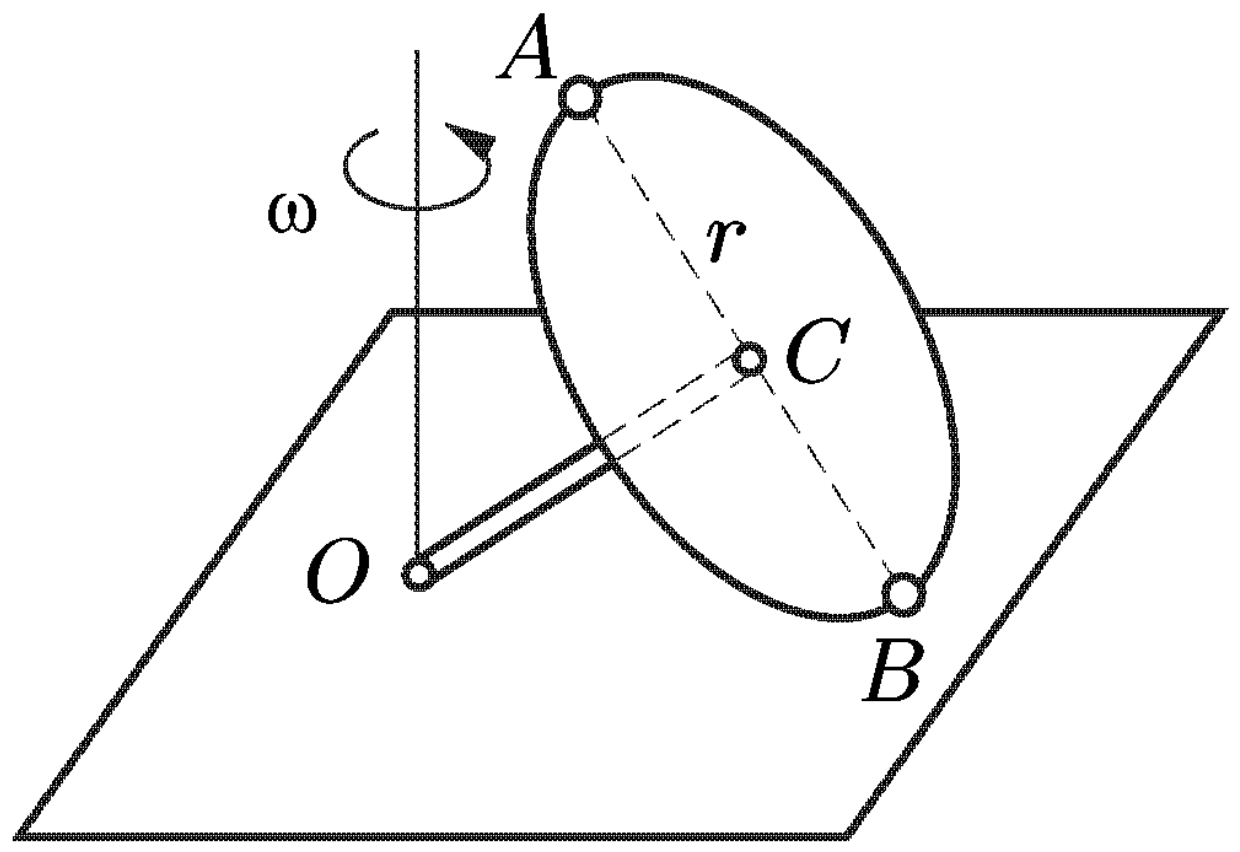
\includegraphics[width=\lw]{4-10}
\end{wrapfigure}
\paragraph{4.10.} Коническое колесо радиуса~$r$, жёстко насаженное
на~стержень~$OC$ длины $l = r\sqrt{3}$, катится по~горизонтальной
плоскости без~скольжения. Стержень~$OC$ описывает коническую поверхность,
вращаясь вокруг неподвижной точки~$O$ (в~точке~$O$ сферический шарнир)
с~угловым ускорением~$\varepsilon$, имея в~данный момент
угловую скорость~$\omega$. Определить угловые скорость и~ускорение
колеса и~ускорения его точек~$A$ и~$B$.

$\blacktriangleright$
Стержень~--- твёрдое тело с~неподвижной точкой~$O$, вращающееся
с~угловой скоростью~$\vec\omega$. С~другой стороны, колесо катится
без~проскальзывания, так~что~$\vec v_B = \overline{0}$.
В~таком случае,
\begin{align}
    \vec v_C &= \vec\omega \times \overline{OC}
        = \vec\Omega \times \overline{BC}; \label{4.10:vC}\\
    \vec w_C &= \vec\varepsilon \times \overline{OC} +
            \vec\omega \times \vec\omega \times \overline{OC}.
\end{align}
где~$\vec\Omega$~--- искомая угловая скорость колеса.
Из~уравнения~\eqref{4.10:vC} найдём её компоненты,
введя правую декартову систему координат~$Oxyz$
(ось~$Ox \upuparrows OB$, ось~$Oz \upuparrows \vec\omega$):
\begin{align}
    \cvec{0}{0}{\omega} \times \cvec{3/2}{0}{\sqrt{3}/2} r &=
            \cvec{\Omega_x}{\Omega_y}{\Omega_z} \times
            \cvec{-1/2}{0}{\sqrt{3}/2} r; \\
    \cvec{0}{3\omega}{0} &=
            \cvec{\sqrt{3}\Omega_y}{\Omega_z-\sqrt{3}\Omega_x}{\Omega_y}.
\end{align}
Видим, что~$\Omega_y = 0$.
Заметим также, что~$\vec v_C = \vec\Omega \times \overline{OC}$,
поскольку колесо движется в~целом как~твёрдое тело:
\begin{align}
    \cvec{0}{\Omega_z - \sqrt{3}\Omega_x}{0} =
            \cvec{\Omega_x}{0}{\Omega_z} \times
            \cvec{3}{0}{\sqrt{3}}
        = \cvec{0}{3\Omega_z - \sqrt{3}\Omega_x}{0}.
\end{align}
Теперь с~необходимостью $\Omega_z = 0$, так~что
$\vec\Omega = -\sqrt{3}\omega \hat x$.

\textsl{Примечание.} Как~направление, так~и~модуль угловой скорости
колеса можно было указать, в~принципе не~совершив никаких вычислений.
С~другой стороны, приведено относительно строгое доказательство
утверждения из~абзаца~1 решения задачи~4.34 (может быть применено
по~аналогии).

Найдём теперь угловое ускорение колеса:
\begin{align}
    \vec{\mathscr{E}} &= \dot{\vec\Omega}
        = -\sqrt{3} \dot\omega \hat x -
            \sqrt{3} \omega \left(\vec\omega \times \hat x\right)
        = -\sqrt{3} \left( \varepsilon \hat x + \omega^2 \hat y \right);
\\
    \mathscr{E} &= \sqrt{3 \left(\varepsilon^2 + \omega^4\right)}.
\end{align}

Ускорения точек~$A$ и~$B$ колеса могут быть рассчитаны
по~формуле Ривальса:
\begin{align}
    \vec w_A &= \vec{\mathscr{E}} \times \overline{OA} +
            \vec\Omega \times \vec\Omega \times \overline{OA}
        = \subst{\overline{OA} = r\hat x + \sqrt{3}r \hat y}
        = \cdots; \label{4.10:wA} \\
    \vec w_B &= \vec{\mathscr{E}} \times \overline{OB} +
            \cancel{\vec\Omega \times \vec\Omega \times \overline{OB}}
        = -\sqrt{3} \left( \varepsilon \hat x + \omega^2 \hat y \right)
            \times 2r \hat x
        = -2\sqrt{3} \omega^2 r. \label{4.10:wB}
\end{align}

\textbf{Ответ:}\quad $\vec{\Omega} = -\sqrt{3}\omega \hat x$;\qquad
$\vec{\mathscr{E}} = -\sqrt{3} \left( \varepsilon \hat x +
\omega^2 \hat y \right)$;\qquad \eqref{4.10:wA} -- \eqref{4.10:wB}.
\hfill $\blacktriangleleft$


\begin{wrapfigure}[13]{l}{6cm}\vspace{-2mm}
    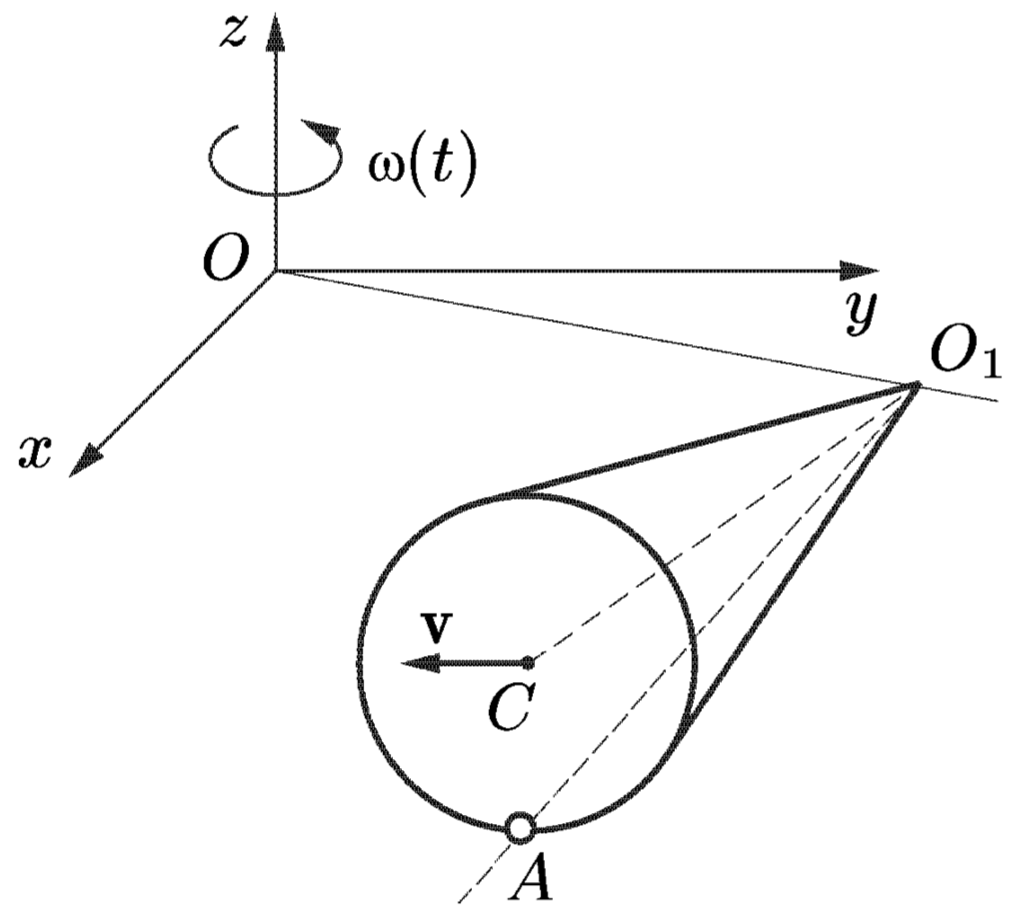
\includegraphics[width=\lw]{4-25}
\end{wrapfigure}
\paragraph{4.25.} Горизонтальная плоскость вращается вокруг
вертикальной оси~$Oz$ с~угловой скоростью~$\omega(t)$.
Конус, вершина~$O_1$ которого неподвижна относительно плоскости,
катится по~ней без~скольжения. Центр основания конуса~$C$
движется равномерно относительно плоскости со~скоростью~$\vec v$.
Найти угловую скорость и~угловое ускорение конуса.
Высота конуса~$h$, угол при~вершине~$2\beta$.

$\blacktriangleright$ Перейдём в~систему отсчёта, вращающуюся
вместе с~плоскостью. В~ней конус совершает мгновенное вращение
с~некоторой угловой скоростью~$\omega_1$ вокруг $O_1A$,
так~что по~формуле Эйлера
\begin{align}
    v = \omega_1 \cdot h \tan\beta
            \sin\left(\frac{\pi}{2} - \beta\right)
        = \omega_1 h \sin\beta.
\end{align}

Вектор~$\vec\omega_1$ вращается в~подвижной системе отсчёта
с~угловой скоростью~$\vec\omega_2$, направленной
против~$Oz$, модуль которой
\begin{equation}
    \omega_2 = \frac{v}{h\cos\beta}.
\end{equation}

В~неподвижной системе отсчёта
\begin{align}
    \vec\Omega &= \vec\omega + \vec\omega_1, &
    \abs{\vec\Omega} &= \sqrt{\omega^2 + \frac{v^2}{h^2\sin^2\beta}};
    \label{4.25:Omega}
\\
    \vec{\mathscr{E}} &= \dot{\vec\omega} +
            \left(\vec\omega + \vec\omega_2\right) \times \vec\omega_1, &
    \abs{\vec{\mathscr{E}}} &= \sqrt{\dot\omega^2 +
            \frac{v^2}{h^2\sin^2\beta}
            \left(\omega - \frac{v}{h\cos\beta}\right)^2}.
    \label{4.25:Eps}
\end{align}

\textbf{Ответ:}\quad \eqref{4.25:Omega} -- \eqref{4.25:Eps}.
\hfill $\blacktriangleleft$


\paragraph{4.29.} При~движении твёрдого тела известны ускорение
точки~$O$ тела~$\vec w_O$, угловая скорость~$\vec\omega$
и~угловое ускорение~$\vec\varepsilon$,
причём~$\vec\omega \times \vec\varepsilon \neq 0$.
Найти точку, ускорение которой равно заданному вектору~$\vec w$.

$\blacktriangleright$ По~формуле Ривальса
\begin{equation}
    \vec w - \vec w_O = \vec\varepsilon \times \vec r +
            \vec\omega \times \vec\omega \times \vec r. \label{4.29:ww}
\end{equation}
Разложим радиус-вектор искомой точки следующим образом:
\begin{equation}
    \vec r = \alpha \vec\omega + \beta \vec\varepsilon +
            \gamma \left[\vec\omega \times \vec\varepsilon\right],
\end{equation}
а~затем подставим последнее выражение в~\eqref{4.29:ww}.

\begin{align}
\begin{split}
    \vec w - \vec w_O &= \vec\varepsilon \times
            \left(\alpha \vec\omega + \beta \vec\varepsilon +
            \gamma \left[\vec\omega \times \vec\varepsilon\right]\right)
            + \vec\omega \times \vec\omega \times
            \left(\alpha \vec\omega + \beta \vec\varepsilon +
            \gamma \left[\vec\omega \times \vec\varepsilon\right]\right)
        =\\&= \alpha \left[\vec\varepsilon \times \vec\omega\right] +
            \gamma \left[\vec\varepsilon \times \vec\omega \times
            \vec\varepsilon\right] + \beta \left[\vec\omega \times
            \vec\omega \times \vec\varepsilon\right] +
            \gamma \left[\vec\omega \times \vec\omega \times \vec\omega
            \times\vec\varepsilon\right] =\\
        &= -\alpha \left[\vec\omega \times \vec\varepsilon\right] +
            \gamma \left(\varepsilon^2 \vec\omega - \vec\varepsilon
            \left(\vec\omega, \vec\varepsilon\right)\right) +
            \beta \left(\vec\omega \left(\vec\omega,
            \vec\varepsilon\right) - \omega^2\vec\varepsilon\right) +\\
        &\qquad+ \gamma\left[\vec\omega \times
            \left(\cancel{\vec\omega \left(\vec\omega,
            \vec\varepsilon\right)} -
            \omega^2\vec\varepsilon\right)\right] =\\
        &= \left\{\gamma\varepsilon^2 + \beta\left(\vec\omega,
            \vec\varepsilon\right)\right\} \vec\omega -
            \left\{\gamma\left(\vec\omega, \vec\varepsilon\right) +
            \beta\omega^2\right\} \vec\varepsilon -
            \left\{\alpha + \gamma\omega^2\right\} \left[\vec\omega
            \times \vec\varepsilon\right].
\end{split}
\end{align}
\begin{align}\tag*{$\blacktriangleleft$}
\begin{cases}
    \gamma\varepsilon^2 + \beta\left(\vec\omega, \vec\varepsilon\right)
        = \dfrac{\left(\vec w - \vec w_O, \vec\omega\right)}{\omega^2};
\\[2ex]
    \gamma\left(\vec\omega, \vec\varepsilon\right) + \beta\omega^2
        = -\dfrac{\left(\vec w - \vec w_O, \vec\varepsilon\right)}
            {\varepsilon^2};
\\[3ex]
    \alpha + \gamma\omega^2 =
        -\dfrac{\left(\vec w - \vec w_O, \vec\omega,
            \vec\varepsilon\right)}
            {\left[\vec\omega \times \vec\varepsilon\right]^2}.
\end{cases}
\end{align}


\paragraph{4.38.} При~движении твёрдого тела, имеющего неподвижную
точку~$O$, углы Эйлера меняются по~закону~$\psi = \omega t$,
$\theta = \pi/3$, $\varphi = 2\omega t$. Определить ускорение
точек~$M$ и~$N$ тела, если~$\overline{OM} \parallel \vec\Omega$,
а~$\overline{ON} \parallel \vec{\mathscr{E}}$,
где~$\vec\Omega$~--- угловая скорость, $\vec{\mathscr{E}}$~--- угловое
ускорение тела. Расстояния $OM = ON = r$.

$\blacktriangleright$
Используем для~решения настоящей задачи кинематические уравнения Эйлера
(в~неподвижных осях~--- \emph{нетрудно вывести}):
\begin{align}
    \vec\Omega &= \cvec{\dot\varphi\sin\theta\sin\psi}
            {-\dot\varphi\sin\theta\cos\psi}
            {\dot\varphi\cos\theta + \dot\psi}
        = \cvec{\sqrt{3}\sin\omega t}
            {-\sqrt{3}\cos\omega t}
            {2} \omega; \\
    \vec{\mathscr{E}} &= \cvec{\cos\psi}{\sin\psi}{0}
            \dot\varphi\dot\psi\sin\theta
        = \cvec{\cos\omega t}{\sin\omega t}{0}
            \sqrt{3}\omega^2.
\end{align}

По~формуле Ривальса
\begin{align}
    \vec w_M &= \vec{\mathscr{E}} \times \overline{OM}
        = \cvec{\cos\omega t}{\sin\omega t}{0} \times
            \cvec{\sqrt{3}\sin\omega t}{-\sqrt{3}\cos\omega t}{2}
            \frac{\sqrt{3} \omega^2 r}{\sqrt{7}}
        = \cvec{2\sin\omega t}{-2\cos\omega t}{-\sqrt{3}}
            \frac{\sqrt{3} \omega^2 r}{\sqrt{7}}, \\
\begin{split}
    \vec w_N &= \vec\Omega \times \vec\Omega \times \overline{ON}
        = \cvec{\sqrt{3}\sin\omega t}{-\sqrt{3}\cos\omega t}{2} \times
            \cvec{\sqrt{3}\sin\omega t}{-\sqrt{3}\cos\omega t}{2} \times
            \cvec{\cos\omega t}{\sin\omega t}{0} \omega^2 r =\\
        &= \cvec{\sqrt{3}\sin\omega t}{-\sqrt{3}\cos\omega t}{2} \times
            \cvec{-2\sin\omega t}{2\cos\omega t}{\sqrt{3}} \omega^2 r
        = \cvec{-7\cos\omega t}{-7\sin\omega t}{0} \omega^2 r; \\[1ex]
    \abs{\vec w_M} &= \sqrt{3}\omega^2 r, \qquad
    \abs{\vec w_N} = 7\omega^2 r.
\end{split}
\end{align}

\textbf{Ответ:}\quad $w_M = \sqrt{3}\omega^2 r$;\qquad
$w_N = 7\omega^2 r$. \hfill $\blacktriangleleft$


\begin{wrapfigure}[9]{l}{4.7cm}
    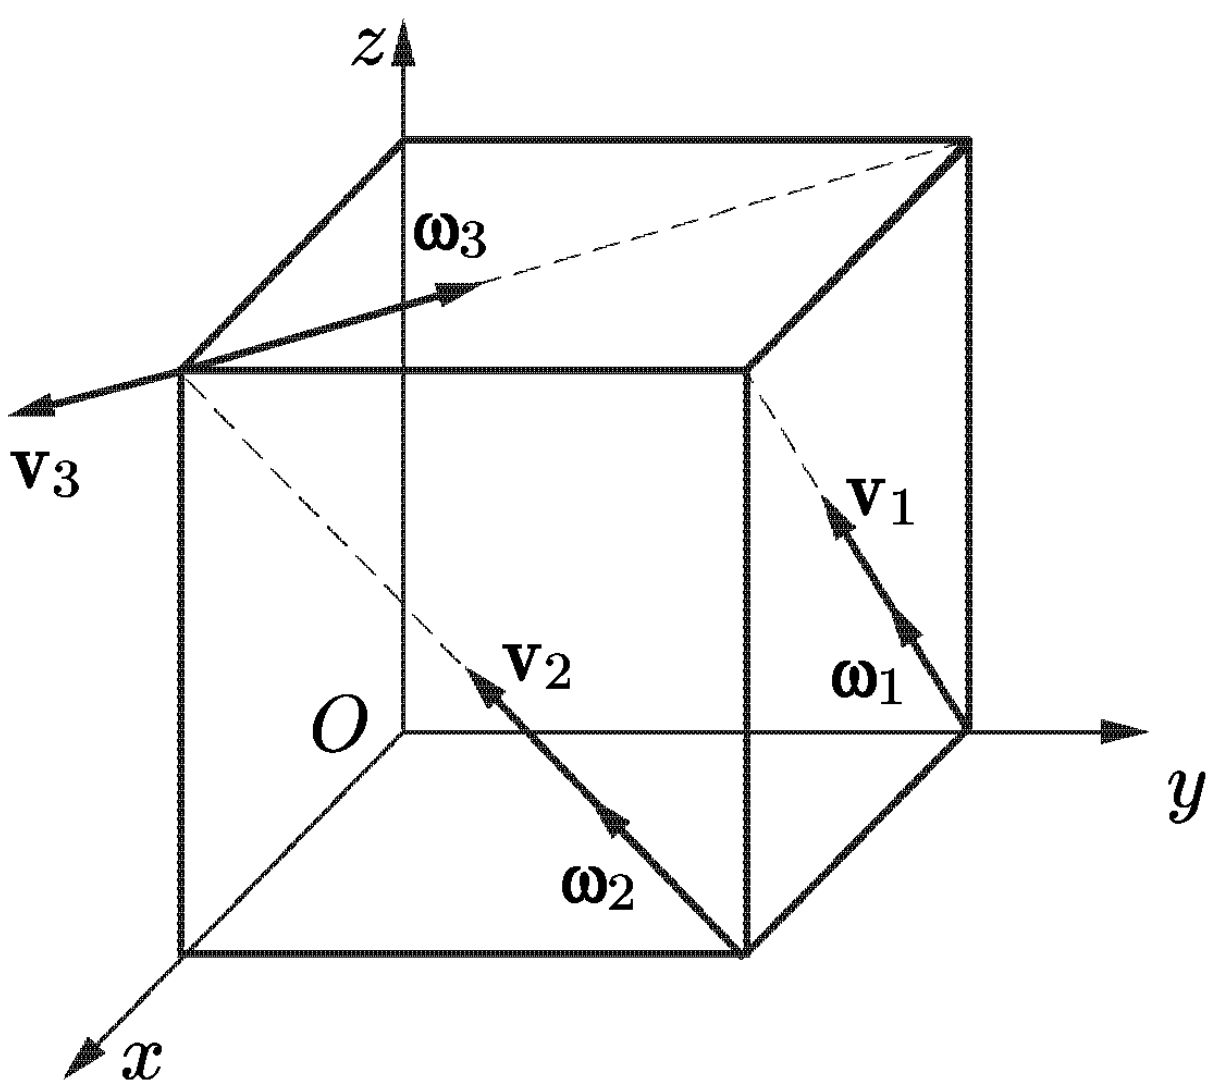
\includegraphics[width=\lw]{4-45}
\end{wrapfigure}
\paragraph{4.45.} Тело участвует одновременно в~трёх винтовых
движениях, оси которых расположены по~диагоналям граней куба
(см.~рис.). Найти результирующее движение тела, если
$\abs{\vec\omega_i} = \omega$, $\abs{\vec v_i} = v$.
Ребро куба равно~$a$.

$\blacktriangleright$ Рассмотрим произвольную точку тела~$A$
и~найдём её скорость:
\begin{align}
\begin{split}
    \vec v_A &= \vec v_1 + \vec\omega_1 \times \vec r_{1A} +
            \vec v_2 + \vec\omega_2 \times \vec r_{2A} +
            \vec v_3 + \vec\omega_3 \times \vec r_{3A} = \\
        &= \left(\vec v_1 + \vec v_2 + \vec v_3 +
            \vec\omega_2 \times \vec r_{21} +
            \vec\omega_3 \times \vec r_{31}\right) +
            \left(\vec\omega_1 + \vec\omega_2 + \vec\omega_3\right)
            \times \vec r_{1A}.
\end{split}
\end{align}
Выберем для~определённости в~качестве рассматриваемой точки полюс~$O$
и~проведём некоторые вычисления:
\begin{align}
    \vec\omega_1 + \vec\omega_2 + \vec\omega_3 &=
            \left[ \cvec{1/\sqrt{2}}{0}{1/\sqrt{2}} +
            \cvec{0}{-1/\sqrt{2}}{1/\sqrt{2}} +
            \cvec{-1/\sqrt{2}}{1/\sqrt{2}}{0} \right] \omega
        = \cvec{0}{0}{\sqrt{2}} \omega; \label{4.45:omegasum}
\\
\begin{split}
    \vec v_O &= \left[ \cvec{1/\sqrt{2}}{0}{1/\sqrt{2}} +
            \cvec{0}{-1/\sqrt{2}}{1/\sqrt{2}} +
            \cvec{1/\sqrt{2}}{-1/\sqrt{2}}{0} \right] v ~+\\
        &+ \left[ \cvec{0}{-1/\sqrt{2}}{1/\sqrt{2}} \times
            \cvec{-1}{0}{0} + \cvec{-1/\sqrt{2}}{1/\sqrt{2}}{0}
            \times \cvec{-1}{1}{-1} + \cvec{0}{0}{\sqrt{2}} \times
            \cvec{0}{-1}{0} \right] \omega a = \\
        &= \sqrt{2} \cvec{1}{-1}{1} v +
            \frac{1}{\sqrt{2}} \cvec{1}{-2}{-1} \omega a
        = \cvec{2v + \omega a}{-2v - 2\omega a}{2v - \omega a}
            \Big/ \sqrt{2}.
\end{split}
\end{align}

Ищем кинематический винт:
\begin{equation}
    \vec v_O + \vec\omega \times \overline{OS} = p\vec\omega,
\end{equation}
где~$S$~--- точка на~оси винта. Это~--- уравнение прямой.
Запишем его в~более определённом, а~лучше~--- каноническом виде:
\begin{equation}
    \frac{v_{Ox} + \left(\xcancel{\omega_y z} - \omega_z y\right)}
        {\xcancel{\omega_x}} =
    \frac{v_{Oy} + \left(\omega_z x - \xcancel{\omega_x z}\right)}
        {\xcancel{\omega_y}} =
    \boxed{\frac{v_{Oz} + \left(\omega_x y - \omega_y x\right)}
        {\omega_z}}.
\end{equation}

\textsl{Примечание.} Результирующая угловая скорость найдена
в~\eqref{4.45:omegasum}, поступательная скорость найдётся
с~учётом связи векторной и~канонической формы уравнения прямой
(нужная часть заключена в~рамку), остальную работу сделала
аналитическая геометрия.

\textbf{Ответ:}\quad винтовое движение с~$\omega' = \sqrt{2}\omega$
и~$v' = \dfrac{2v - \omega a}{\sqrt{2}}$ вокруг
$
\begin{cases}
    x = \dfrac{v}{\omega} + a; \\[2ex]
    y = \dfrac{v}{\omega} + \dfrac{a}{2}.
\end{cases}
$
\hfill $\blacktriangleleft$


\end{document}
